\documentclass[]{book}
\usepackage{lmodern}
\usepackage{amssymb,amsmath}
\usepackage{ifxetex,ifluatex}
\usepackage{fixltx2e} % provides \textsubscript
\ifnum 0\ifxetex 1\fi\ifluatex 1\fi=0 % if pdftex
  \usepackage[T1]{fontenc}
  \usepackage[utf8]{inputenc}
\else % if luatex or xelatex
  \ifxetex
    \usepackage{mathspec}
  \else
    \usepackage{fontspec}
  \fi
  \defaultfontfeatures{Ligatures=TeX,Scale=MatchLowercase}
\fi
% use upquote if available, for straight quotes in verbatim environments
\IfFileExists{upquote.sty}{\usepackage{upquote}}{}
% use microtype if available
\IfFileExists{microtype.sty}{%
\usepackage{microtype}
\UseMicrotypeSet[protrusion]{basicmath} % disable protrusion for tt fonts
}{}
\usepackage[margin=1in]{geometry}
\usepackage{hyperref}
\hypersetup{unicode=true,
            pdftitle={CAMB 698 Final Paper},
            pdfauthor={Vincent Wu},
            pdfborder={0 0 0},
            breaklinks=true}
\urlstyle{same}  % don't use monospace font for urls
\usepackage{natbib}
\bibliographystyle{apalike}
\usepackage{color}
\usepackage{fancyvrb}
\newcommand{\VerbBar}{|}
\newcommand{\VERB}{\Verb[commandchars=\\\{\}]}
\DefineVerbatimEnvironment{Highlighting}{Verbatim}{commandchars=\\\{\}}
% Add ',fontsize=\small' for more characters per line
\usepackage{framed}
\definecolor{shadecolor}{RGB}{248,248,248}
\newenvironment{Shaded}{\begin{snugshade}}{\end{snugshade}}
\newcommand{\KeywordTok}[1]{\textcolor[rgb]{0.13,0.29,0.53}{\textbf{#1}}}
\newcommand{\DataTypeTok}[1]{\textcolor[rgb]{0.13,0.29,0.53}{#1}}
\newcommand{\DecValTok}[1]{\textcolor[rgb]{0.00,0.00,0.81}{#1}}
\newcommand{\BaseNTok}[1]{\textcolor[rgb]{0.00,0.00,0.81}{#1}}
\newcommand{\FloatTok}[1]{\textcolor[rgb]{0.00,0.00,0.81}{#1}}
\newcommand{\ConstantTok}[1]{\textcolor[rgb]{0.00,0.00,0.00}{#1}}
\newcommand{\CharTok}[1]{\textcolor[rgb]{0.31,0.60,0.02}{#1}}
\newcommand{\SpecialCharTok}[1]{\textcolor[rgb]{0.00,0.00,0.00}{#1}}
\newcommand{\StringTok}[1]{\textcolor[rgb]{0.31,0.60,0.02}{#1}}
\newcommand{\VerbatimStringTok}[1]{\textcolor[rgb]{0.31,0.60,0.02}{#1}}
\newcommand{\SpecialStringTok}[1]{\textcolor[rgb]{0.31,0.60,0.02}{#1}}
\newcommand{\ImportTok}[1]{#1}
\newcommand{\CommentTok}[1]{\textcolor[rgb]{0.56,0.35,0.01}{\textit{#1}}}
\newcommand{\DocumentationTok}[1]{\textcolor[rgb]{0.56,0.35,0.01}{\textbf{\textit{#1}}}}
\newcommand{\AnnotationTok}[1]{\textcolor[rgb]{0.56,0.35,0.01}{\textbf{\textit{#1}}}}
\newcommand{\CommentVarTok}[1]{\textcolor[rgb]{0.56,0.35,0.01}{\textbf{\textit{#1}}}}
\newcommand{\OtherTok}[1]{\textcolor[rgb]{0.56,0.35,0.01}{#1}}
\newcommand{\FunctionTok}[1]{\textcolor[rgb]{0.00,0.00,0.00}{#1}}
\newcommand{\VariableTok}[1]{\textcolor[rgb]{0.00,0.00,0.00}{#1}}
\newcommand{\ControlFlowTok}[1]{\textcolor[rgb]{0.13,0.29,0.53}{\textbf{#1}}}
\newcommand{\OperatorTok}[1]{\textcolor[rgb]{0.81,0.36,0.00}{\textbf{#1}}}
\newcommand{\BuiltInTok}[1]{#1}
\newcommand{\ExtensionTok}[1]{#1}
\newcommand{\PreprocessorTok}[1]{\textcolor[rgb]{0.56,0.35,0.01}{\textit{#1}}}
\newcommand{\AttributeTok}[1]{\textcolor[rgb]{0.77,0.63,0.00}{#1}}
\newcommand{\RegionMarkerTok}[1]{#1}
\newcommand{\InformationTok}[1]{\textcolor[rgb]{0.56,0.35,0.01}{\textbf{\textit{#1}}}}
\newcommand{\WarningTok}[1]{\textcolor[rgb]{0.56,0.35,0.01}{\textbf{\textit{#1}}}}
\newcommand{\AlertTok}[1]{\textcolor[rgb]{0.94,0.16,0.16}{#1}}
\newcommand{\ErrorTok}[1]{\textcolor[rgb]{0.64,0.00,0.00}{\textbf{#1}}}
\newcommand{\NormalTok}[1]{#1}
\usepackage{longtable,booktabs}
\usepackage{graphicx,grffile}
\makeatletter
\def\maxwidth{\ifdim\Gin@nat@width>\linewidth\linewidth\else\Gin@nat@width\fi}
\def\maxheight{\ifdim\Gin@nat@height>\textheight\textheight\else\Gin@nat@height\fi}
\makeatother
% Scale images if necessary, so that they will not overflow the page
% margins by default, and it is still possible to overwrite the defaults
% using explicit options in \includegraphics[width, height, ...]{}
\setkeys{Gin}{width=\maxwidth,height=\maxheight,keepaspectratio}
\IfFileExists{parskip.sty}{%
\usepackage{parskip}
}{% else
\setlength{\parindent}{0pt}
\setlength{\parskip}{6pt plus 2pt minus 1pt}
}
\setlength{\emergencystretch}{3em}  % prevent overfull lines
\providecommand{\tightlist}{%
  \setlength{\itemsep}{0pt}\setlength{\parskip}{0pt}}
\setcounter{secnumdepth}{5}
% Redefines (sub)paragraphs to behave more like sections
\ifx\paragraph\undefined\else
\let\oldparagraph\paragraph
\renewcommand{\paragraph}[1]{\oldparagraph{#1}\mbox{}}
\fi
\ifx\subparagraph\undefined\else
\let\oldsubparagraph\subparagraph
\renewcommand{\subparagraph}[1]{\oldsubparagraph{#1}\mbox{}}
\fi

%%% Use protect on footnotes to avoid problems with footnotes in titles
\let\rmarkdownfootnote\footnote%
\def\footnote{\protect\rmarkdownfootnote}

%%% Change title format to be more compact
\usepackage{titling}

% Create subtitle command for use in maketitle
\newcommand{\subtitle}[1]{
  \posttitle{
    \begin{center}\large#1\end{center}
    }
}

\setlength{\droptitle}{-2em}

  \title{CAMB 698 Final Paper}
    \pretitle{\vspace{\droptitle}\centering\huge}
  \posttitle{\par}
    \author{Vincent Wu}
    \preauthor{\centering\large\emph}
  \postauthor{\par}
      \predate{\centering\large\emph}
  \postdate{\par}
    \date{2018-12-09}

\usepackage{booktabs}

\begin{document}
\maketitle

{
\setcounter{tocdepth}{1}
\tableofcontents
}
\chapter{Prerequesites}\label{prerequesites}

This book will feature code and graphs produced using the R statistical
language. Below are packages that will be used throughout this book.

\begin{Shaded}
\begin{Highlighting}[]
\KeywordTok{library}\NormalTok{(tidyverse)}
\KeywordTok{library}\NormalTok{(usedist)}
\KeywordTok{library}\NormalTok{(qiimer)}
\KeywordTok{library}\NormalTok{(reshape2)}
\KeywordTok{library}\NormalTok{(ggplot2)}

\KeywordTok{library}\NormalTok{(ape)}
\KeywordTok{library}\NormalTok{(Rtsne)}
\end{Highlighting}
\end{Shaded}

The below code will load in the data that will be used in the next
sections.

\begin{Shaded}
\begin{Highlighting}[]
\KeywordTok{load}\NormalTok{(}\StringTok{"data/poop_across_penn1.Rdata"}\NormalTok{)}
\end{Highlighting}
\end{Shaded}

\begin{Shaded}
\begin{Highlighting}[]
\CommentTok{# Create vendor/mice dataframe}
\NormalTok{s_vendor_all <-}\StringTok{ }\NormalTok{s }\OperatorTok
\StringTok{  }\KeywordTok{filter}\NormalTok{(}\KeywordTok{grepl}\NormalTok{(}\StringTok{"ARC Vendor Experiment"}\NormalTok{, Experiment)) }\OperatorTok
\StringTok{  }\KeywordTok{rename}\NormalTok{(}\DataTypeTok{Vendor =}\NormalTok{ Mouse_Source_Vendor) }\OperatorTok
\StringTok{  }\KeywordTok{mutate}\NormalTok{(}\DataTypeTok{SubjectID =} \KeywordTok{factor}\NormalTok{(}\KeywordTok{paste}\NormalTok{(}\StringTok{"Mouse"}\NormalTok{, Mouse_Number))) }\OperatorTok
\StringTok{  }\KeywordTok{mutate}\NormalTok{(}\DataTypeTok{SampleType =} \KeywordTok{trimws}\NormalTok{(}\KeywordTok{as.character}\NormalTok{(SampleType))) }\OperatorTok
\StringTok{  }\KeywordTok{arrange}\NormalTok{(SampleType, Vendor, SubjectID)}

\CommentTok{# Identify and remove suspicious samples}
\NormalTok{suspect_SampleIDs <-}\StringTok{ }\KeywordTok{c}\NormalTok{(}\StringTok{"Tac.33.CE.Day1"}\NormalTok{, }\StringTok{"Env.13.Stool.Day0"}\NormalTok{)}

\CommentTok{# Set final dataframe}
\NormalTok{s_vendor <-}\StringTok{ }\NormalTok{s_vendor_all }\OperatorTok
\StringTok{  }\KeywordTok{droplevels}\NormalTok{() }\OperatorTok
\StringTok{  }\KeywordTok{filter}\NormalTok{(}\OperatorTok{!}\NormalTok{(SampleID }\OperatorTok\StringTok{ }\NormalTok{suspect_SampleIDs))}
\end{Highlighting}
\end{Shaded}

\chapter{Background}\label{bg}

From the initial raw data to visualizing the results, data processing
and analysis are fundamental aspects of conducting scientific research.
With the recent advances of high throughput technologies (i.e.~the many
``-omics'', multiparametric flow cytometry, etc.), the accompanying data
is often high-dimensional and difficult for manual efforts to analyze.
The development of machine learning methods aims to help with this
problem, thus helping to make sense of the data to draw meaningful and
accurate conclusions.

The purpose of this paper is to introduce and explore the different
machine learning methods that are commonly used in the biological
sciences. To help demonstrate the methods and to maintain the same
context across all of the methods, a single dataset (will be referred to
as the PAP dataset) was provided by the PennCHOP Microbiome Program
(courtesy of Dr.~Kyle Bittinger). Mice were purchased from vendors with
the purpose of assessing whether the mice have different phenotypes from
different vendors. The fecal microbiota was sequenced from the mice,
resulting in a distance matrix (how distant each mouse's microbiome was
from the other mice sampled) as well as the relative abundance of
bacterial species for each mouse. Additionally, metabolites as well as
different immune phenotypes were assessed for each mouse. This
high-dimensional dataset is representative of datasets that are seen
with microbiome research.

\chapter{Dimensionality reduction}\label{dim_red}

\section{Introduction to dimensionality
reduction}\label{introduction-to-dimensionality-reduction}

Dimensionality reduction is a necessary tool for working with
high-dimensional data, which can be seen from this dataset. Each of the
diversity distances against each of the mice is a single variable, as is
each of the relative abundances for different species. A variable is a
dimension in this scenario -- creating a dataset with hundreds of
dimensions. While rich and informative, this dataset would be difficult
to visualize beyond two dimensions. Without going too far into the
mathematics behind these methods, dimensionality reduction creates a
means to observe the data from a different perspective and assists in
reducing the computational burden for the machine learning techniques
that will be discussed.

\section{PCA and PCoA}\label{pca-and-pcoa}

Principal components analysis (PCA) and principal coordinates analysis
(PCoA) are common techniques used both in and outside of the biological
sciences. PCA makes new variables that are linear combinations of the
original variables. PCoA is similar in concept but takes in a distance
matrix (such as the one used for our dataset) to transform into new
coordinates where the axes of this coordinate system are not correlated
with each other. The power of PCA and PCoA is that all new variables
have no correlation with each other and can explain all the covariance
from the original data. The data points in PCA or PCoA space can be
easily visualized as seen in the below graph. It is common to display
the variance explained by each of the principal component axes as a
means to show how well the principal components can explain the variance
in the original data.

\subsection{PCoA example}\label{pcoa-example}

\begin{Shaded}
\begin{Highlighting}[]
\CommentTok{# get unweighted unifrac distances}
\NormalTok{uu <-}\StringTok{ }\KeywordTok{dist_subset}\NormalTok{(uu, s_vendor}\OperatorTok{$}\NormalTok{SampleID)}

\CommentTok{# run pcoa}
\NormalTok{pc <-}\StringTok{ }\KeywordTok{pcoa}\NormalTok{(uu)}

\CommentTok{# create dataframe for ggplot2}
\NormalTok{pc_df_uu <-}\StringTok{ }\KeywordTok{cbind}\NormalTok{(s_vendor, pc}\OperatorTok{$}\NormalTok{vectors[s_vendor}\OperatorTok{$}\NormalTok{SampleID,}\DecValTok{1}\OperatorTok{:}\DecValTok{3}\NormalTok{])}

\CommentTok{# calculate variance coverage by axis}
\NormalTok{pc_pct <-}\StringTok{ }\KeywordTok{round}\NormalTok{(pc}\OperatorTok{$}\NormalTok{values}\OperatorTok{$}\NormalTok{Relative_eig }\OperatorTok{*}\StringTok{ }\DecValTok{100}\NormalTok{)}

\CommentTok{# finish setting up dataframe}
\NormalTok{pc_df_uu <-}\StringTok{ }\NormalTok{pc_df_uu }\OperatorTok
\StringTok{  }\KeywordTok{mutate}\NormalTok{(}\DataTypeTok{Label =} \KeywordTok{ifelse}\NormalTok{(SampleID }\OperatorTok\StringTok{ }\NormalTok{suspect_SampleIDs, SampleID, }\StringTok{""}\NormalTok{))}

\CommentTok{# make fig}
\KeywordTok{ggplot}\NormalTok{(pc_df_uu, }\KeywordTok{aes}\NormalTok{(}\DataTypeTok{x =}\NormalTok{ Axis.}\DecValTok{1}\NormalTok{, }\DataTypeTok{y =}\NormalTok{ Axis.}\DecValTok{2}\NormalTok{)) }\OperatorTok{+}
\StringTok{  }\KeywordTok{geom_point}\NormalTok{(}\KeywordTok{aes}\NormalTok{(}\DataTypeTok{color =}\NormalTok{ Vendor, }\DataTypeTok{shape =}\NormalTok{ SampleType)) }\OperatorTok{+}
\StringTok{  }\KeywordTok{geom_text}\NormalTok{(}\KeywordTok{aes}\NormalTok{(}\DataTypeTok{label =}\NormalTok{ Label)) }\OperatorTok{+}
\StringTok{  }\KeywordTok{labs}\NormalTok{(}
    \DataTypeTok{title =} \StringTok{"PCoA plot of Unweighted Unifrac Distances across Mice"}\NormalTok{,}
    \DataTypeTok{x =} \KeywordTok{paste0}\NormalTok{(}\StringTok{"PCoA Axis 1 ("}\NormalTok{, pc_pct[}\DecValTok{1}\NormalTok{], }\StringTok{"%)"}\NormalTok{),}
    \DataTypeTok{y =} \KeywordTok{paste0}\NormalTok{(}\StringTok{"PCoA Axis 2 ("}\NormalTok{, pc_pct[}\DecValTok{2}\NormalTok{], }\StringTok{"%)"}\NormalTok{)) }\OperatorTok{+}
\StringTok{  }\KeywordTok{theme_classic}\NormalTok{()}
\end{Highlighting}
\end{Shaded}

\begin{figure}
\centering
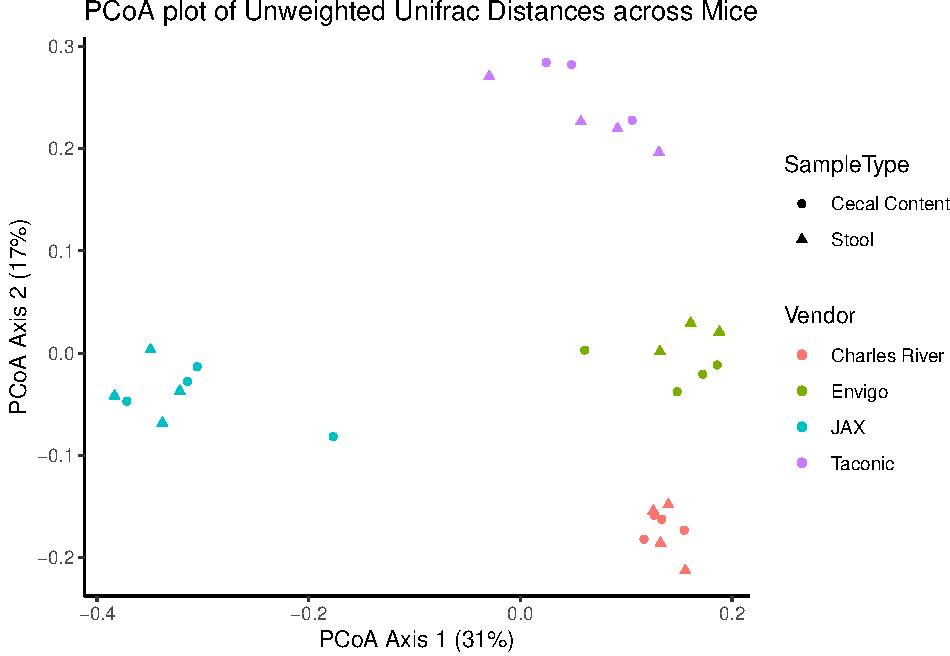
\includegraphics{final_paper_files/figure-latex/unnamed-chunk-4-1.pdf}
\caption{\label{fig:unnamed-chunk-4}PCoA plot}
\end{figure}

\bibliography{book.bib,packages.bib}


\end{document}
